% ********** Chapter 1 **********
\chapter{Background}
\label{ch1}

Before implementing a sociotechnical system, we need to understand what a sociotechnical system is and its characteristics, problems in the system and possible solutions of the problems. Whitworth and Ahmad \cite{whitworth2013} claimed a sociotechnical system as a social system operating on a technical base, such as email, chat, Facebook, and described the design process of a sociotechnical system. Why do we need a sociotechnical system instead of a common computer-based or technical system? As Baxter and Sommerville \cite{baxter2011} stated, systems often meet their technical "requirements" but are considered to be a "failure" because they do not deliver the expected support for the real work in the organization. The source of the problem is that techno-centric approaches to systems design do not properly consider the complex relationships between the organization, the people enacting business processes and the system that supports these processes.

In this chapter, first we present background knowledge of sociotechnical systems, including the concept and some keywords related to our work. Then we introduce a complex problem of sociotechnical systems that is related to our case studies here - the resource allocation problem. At last, multiagent systems are introduced to tackle the problems in a sociotechnical system.  

\section{Sociotechnical Systems}
\label{ch1:sociotechnicalSys}
For solving complex problems, we should understand the environment that the problems build on, i.e., different kinds of sociotechnical systems. Today everyone lives in some sociotechnical systems one way or another. The name "SocioTechnical Systems" indicates both the social aspects, such as humans or society, and the technical aspects, such as organizational rules and policies in the system. Through interaction and cooperation of all the participants in the system, it is expected to achieve solutions better than that achieved with only technology or humans available in the system. Let's consider some examples on top of the find-a-doctor example mentioned before. 

Sociotechnical systems are common and play an important role in our era due to increasingly complex societies, which rely on increased connectivity and global interactions between humans and technology. Information globalization changes human life in many ways, from communication between friends, to the way the companies operate their business. All these require the cooperation of the social and technical aspects. Take companies as an example, as Valacich \cite{valacich2009information} stated, information technology is important because "increasing global competitiveness has forced companies to find ways to be better and to do things less expensively. The answer for many firms continues to be to use information systems to do things better, faster, and cheaper. Using global telecommunications networks, companies can more easily integrate their operations to access new markets for their products and services as well as access a large pool of talented labor in countries with lower wages." Thus, sociotechnical systems are formed and used to deal with different situations. 

Figure \ref{ch1:fmodelsocio} shows the model of a sociotechnical system. In the rectangle marked with "network" there are humans represented by their individual agents involved in a particular event forming a network. In the network, agents representing their principles could communicate with each other. Meanwhile, agents could also upload or download information from a database under the control of a central manager in the cloud, who is also an agent with a different functionality. The black robot in the figure is the central manager and the cylinder besides it represents the database it manages. 

\begin{figure}
\centering
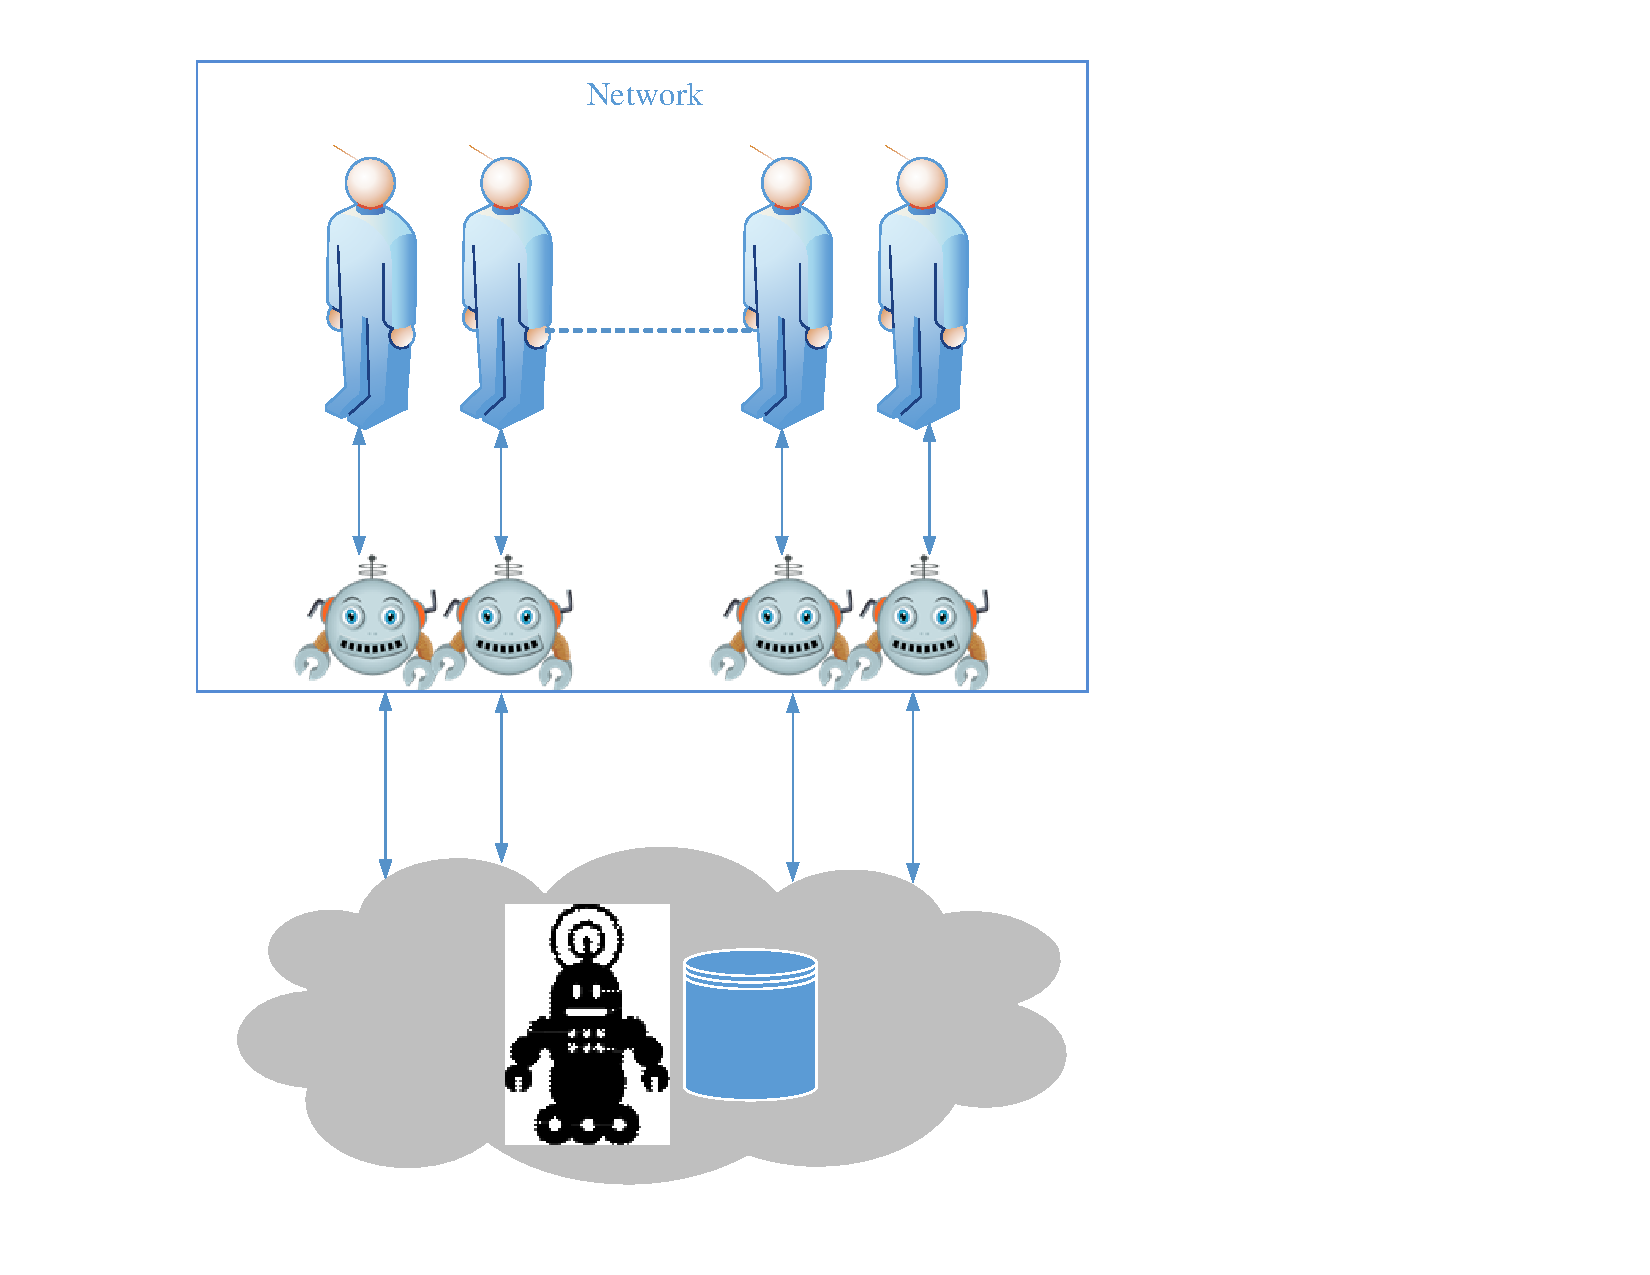
\includegraphics[scale=0.5]{chap1/chap1-model.pdf}
\caption{The model of a sociotechnical system}
\label{ch1:fmodelsocio}
\end{figure}

Problems arise from complex sociotechnical systems. To analyze these problems, simulated systems are built. Why do we use simulated systems rather than real-world systems? There are a couple of reasons. One is that using simulation would cost less. For example, if you want to do an experiment with a hundred people, you'll have to gather subjects, tell them the rules, and do the experiment at a specific time. If you want to check the influence of the parameters in your system, you'll need to ask the subjects to do the experiment multiple times. All these experiments in real-world systems cost time and energy. Another reason is that sometimes the sociotechnical systems are so complex that it's hard to perform experiments in the real-world. Simulations costs less and can mimic extreme conditions. Meanwhile, it could be a good imitation of the real-world situation if modeled well. Then computational methodologies are used to analyze and solve these problems. One of these advanced methods is to use multiagent systems, which will be introduced in section \ref{ch1:mas}.

\subsection{Norms}
\label{ch1:norms}

An important concept in a sociotechnical system or a multiagent system is norms. Norms regulate the interaction of agents by specifying rules of encounter and lead the way of how each principle should behave under certain circumstances. Bicchieri \cite{bicchieri1990} defines a social norm (N) in a population (P) as a function of the beliefs and preferences of the members of P is the following conditions hold:
\begin{itemize}
\item[-]Almost every member of P prefers to conform to N on the condition that almost everyone else conforms, too.
\item[-]Almost every member of P believes that almost every other member of P conforms to N.
\end{itemize}
The definition suggests that a social norm is an equilibrium in the game-theoretic sense.  

Norms are used in the multiagent systems to regulate the behavior of the autonomous agents \cite{boella2009} \cite{hollander2011}. For example, Hexmoor \cite{hexmoor2006} modeled norms in multiagent systems and defined an account of norm stability; Singh \cite{singh2014} viewed a sociotechnical system as a multistakeholder cyber-physical system and developed an approach for governance based on a computational representation of norms in organizations.

Norms could be used in our systems. In the grocery shopping scenario, for updating goods data in the center server, customers are expected to upload real information, otherwise they get punished, for example, by rated as "low confidence". In the health care scenario, a patient's agent trusts the information of other agents if they respond, which means the norms here include that the agents should not lie to each other. In the human-agent interaction case, we expect that the simulated human and the agent in the game don't lure the subject to make biased decisions.    

\subsection{Crowdsourcing}
\label{ch1:crowdsourcing}

One of the most promising approach to solve complex problems in sociotechnical systems is to use crowdsourcing, which is a distributed methodology. Here is the definition from Howe \cite{crowdsourcing}, who coined the word "crowdsourcing" in 2006: "crowdsourcing represents the act of a company or institution taking a function once performed by employees and outsourcing it to an undefined (and generally large) network of people in the form of an open call. This can take the form of peer-production (when the job is performed collaboratively), but is also often undertaken by sole individuals. The crucial prerequisite is the use of the open call format and the large network of potential laborers." 

Crowdsourcing is used by large companies, such as Amazon and Google. Amazon's crowdsourcing platform, Amazon Mechanical Turk (AMT), allows people to post or process tasks on the platform. Companies could use crowdsourcing to receive solutions quickly at relatively little cost \cite{satzger2013} \cite{skopik2012}. One problem that a crowdsourcing system designer should concern is the incentives \cite{mason2009} \cite{tokarchuk2012} \cite{scekic2013}.

We kind of borrow the concept of crowdsourcing in our first two case studies, but use it in a different way: both utilize the power of the crowd. In the grocery shopping scenario, we may rely on the goods information reported by customers. In the health care system, information related to physicians is passed through the network of agents and is integrated later. 

\subsection{Mixed Human-Agent Societies}    
\label{ch1:mixedHumAgeSoc}
As we mentioned earlier, due to the enormous participation of agents into human societies, mixed human-agent societies are formed. For example, "social computers" which combine software and human services are constructed. Truong et al. \cite{truong2013} \cite{truong2012} propose a method to model human capabilities using cloud computing concepts and combine it with software-based services and establish clouds of hybrid services. Sierhuis et al. \cite{bradshaw2003} use a human-centered perspective on teamwork and adjustable autonomy in mixed human-agent groups and integrate the Brahms \cite{clancey1998} and KAoS \cite{uszok2004} agent frameworks to model real work situations. 

Because of the challenges in human-agent teamwork coordination \cite{bradshaw2008}, we want to explore ways that could improve the coordination. Among many perspectives or aspects that can be used to improve coordination, we particularly look into a psychological factor: personality in the third case study in the hope of understanding humans' attitude towards agents better and expecting conclusions that could be utilized in human-agent interactions.       

\section{Resource Allocation Problems}
\label{ch1:resourceAllPro}

There is a lot of concerns on resource allocation problems in both computer science and economics fields, especially when the resource is scarce. There are circumstances under which we need to distribute different kinds of resources, such as electricity, water, network bandwidth, among multiple entities or agents. A particular distribution of the resource is called an allocation. Since multiple agents are involved, resource allocation problems are also called \emph{MultiAgent Resource Allocation (MARA)} problems.

Multiagent Resource allocation has a wide range of applications, such as manufacturing and scheduling \cite{lee2009} \cite{adhau2012}, logistics \cite{santos2003} and so on. Chevaleyre et al. \cite{chevaleyre2006} presented techniques, concepts, and four major application domains of MARA: industrial procurement, the joint exploitation of Earth Observation Satellites, manufacturing control, and grid computing. Feldman, Lai, and Zhang \cite{feldman2005} proposed a distributed allocation scheme that converged quickly to an equilibrium while maintaining the balance of efficiency and the fairness indicated by utility uniformity and envy-freeness. Some researchers developed resource allocation algorithms related to cloud computing. For example, Ergu et al. \cite{ergu2013} proposed a model for task-oriented resource allocation in a cloud computing environment with ranking and a bias matrix was used to solve conflicts. In wireless networks, power, time slots, etc. are the resources that need to be allocated \cite{eryilmaz2007} \cite{altman2010} \cite{wang2011}.   

In game theory, auction is an important mechanism to provide a general solution to discrete resource allocation among selfish agents. Formally speaking, an auction is any protocol that allows agents to indicate their interests in one or more resources and that uses these indications of interest to determine both an allocation  resources and a set of payments by the agents \cite{shoham2008}.

The allocation procedure could be centralized or distributed. A centralized procedure requires a single entity that receives the agents' preferences and chooses an outcome that satisfies a certain condition, such as maximizing social welfare. One problem is that agents may lie about their private information, which happens very common in a collaborative environment \cite{malik2012} \cite{malik2010}. Also, it may not always be possible to establish a central entity. A distributed procedure doesn't need the central entity and usually involves negotiation among the agents. Schmidt et al. \cite{schmidt2009} discussed different distributed resource allocation schemes. Bachrach and Rosenschein \cite{bachrach2008} proposed a distributed and random allocation procedure that converged to the optimal in terms of utilitarian social welfare.

The third case study is related to resource allocation. It asks the participants to play a "Who Gets More Cake?" game which is a variant of cake-cutting resource allocation game with a human-agent related question at the end of the game. 

\section{Multiagent Systems}
\label{ch1:mas}

Researchers proposed different definitions about an agent, or an intelligent agent \cite{muller1997}. According to Russell and Norvig \cite{russell2009}, an agent is anything that can be viewed as perceiving its environment through sensors and acting upon that environment through effectors. Jennings, Sycara and Wooldridge \cite{jennings1998} consider an agent as a computer system, situated in some environment, that is capable of flexible autonomous action in order to meet its design objectives.

All the definitions agree that an agent should be intelligent and autonomous that he could make decisions and act on the principle's behalf on his own based on the environment he perceived \cite{jennings1998} \cite{russell2009} \cite{wooldridge2009}, as shown in Figure \ref{ch1:fagent}. An agent could be simple, such as a thermostat which controls the air conditioner of a room and keeps the temperature stable, or something very complex, such as a robot which acts according to the environment and tries to achieve predefined goals. The thermostat perceives information about the environment using the mechanic part that detects the temperature and achieves the goal of keeping the room temperature stable by turning on/off the air conditioner. The robot perceives the environment using cameras and other sensors and takes action, e.g., moving to a specific location, based on the information he integrated. Interestingly, a human could be treated as an agent with organs perceiving the environment and a brain that integrates perceived information and makes decisions. 

\begin{figure}
\centering
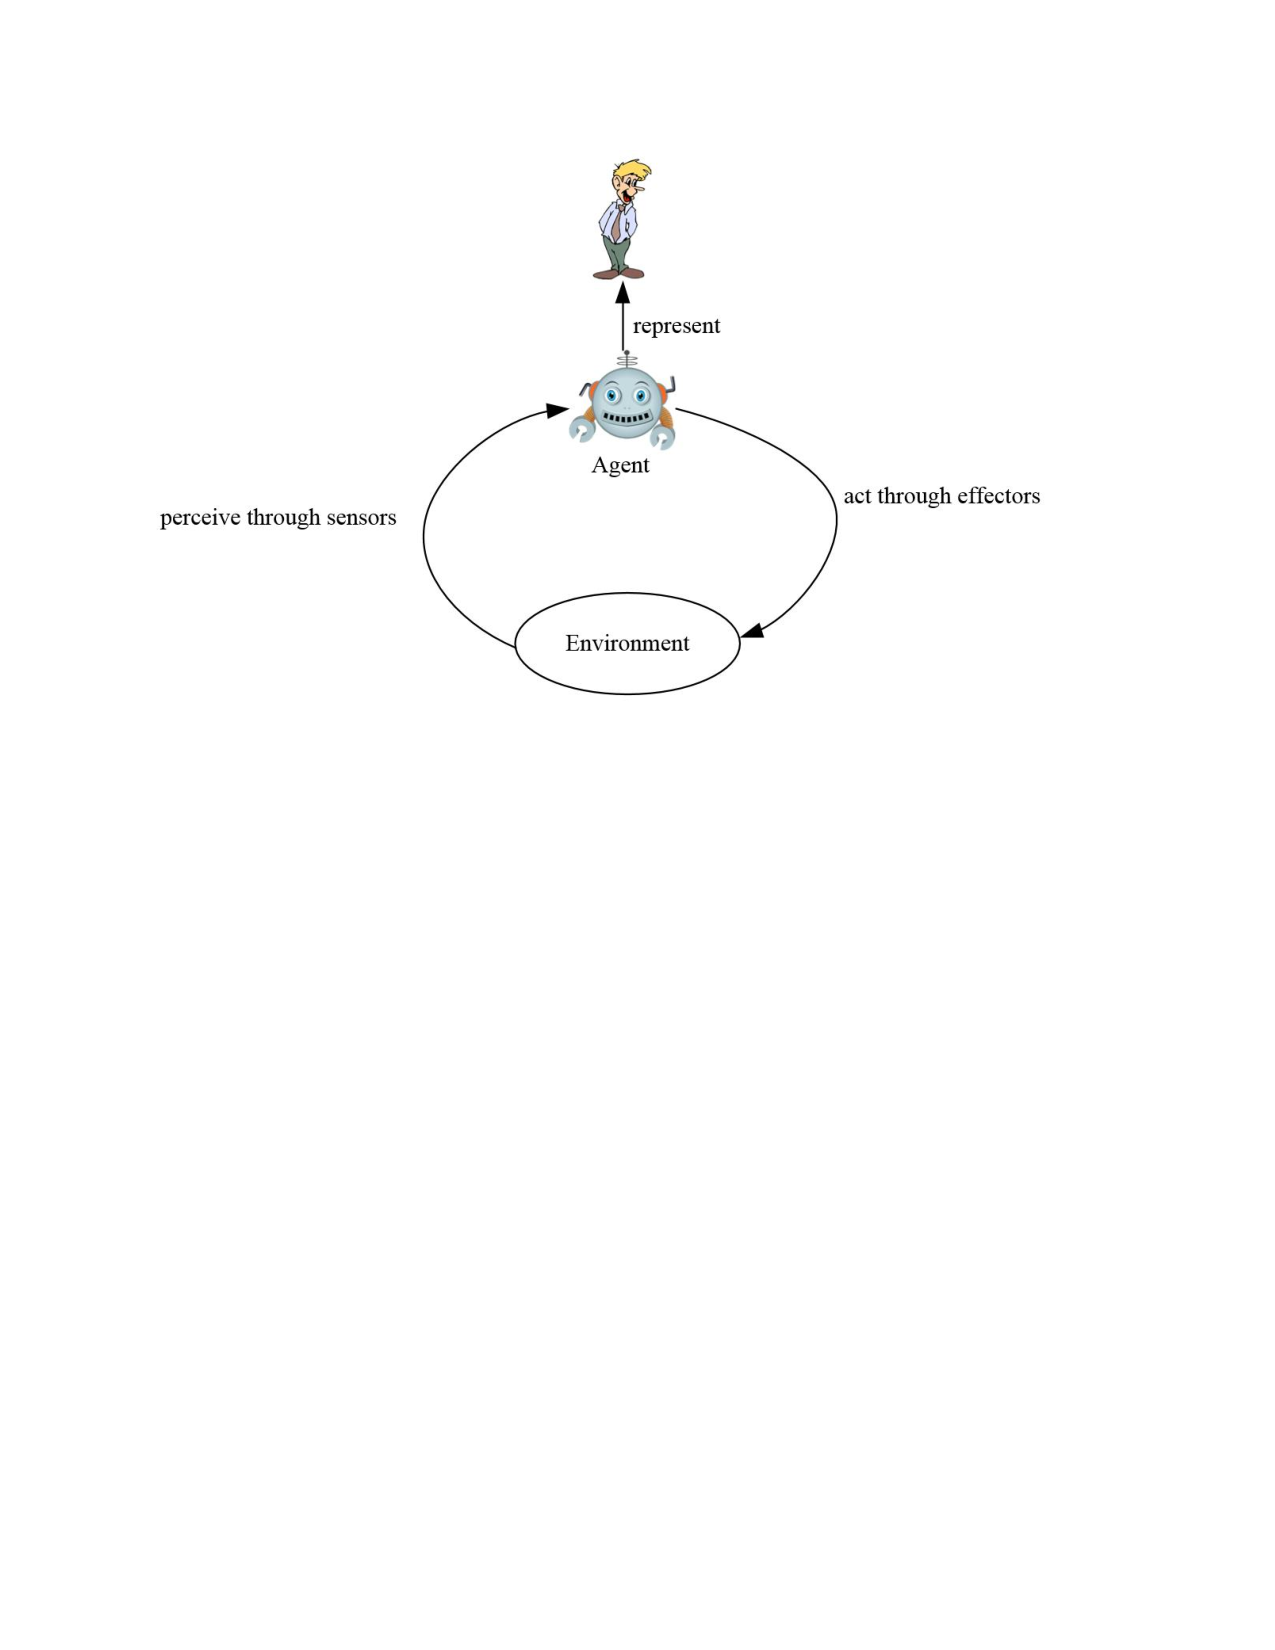
\includegraphics[scale=0.8]{chap1/chap1-agent.pdf}
\caption{The model of an agent}
\label{ch1:fagent}
\end{figure}

There are a couple of features that an agent could have \cite{jennings1998}, while autonomy is the central notion of agency.
\begin{itemize}
\item[-]situatedness: the agent receives sensory input from its environment and it can perform actions which change the environment in some way.
\item[-]autonomy: in the sense that the system should be able to act without the direct intervention of humans or other agents.
\item[-]flexibility: which contains the following three factors:
\begin{itemize}
\item[-]responsive: the agent should perceive their environment and respond in a timely fashion to changes that occur in it.
\item[-]pro-active: the agent should be able to exhibit opportunistic, goal-directed behavior and take the initiative where appropriate.
\item[-]social: the agent should be able to interact, when appropriate, with other artificial agents and humans in order to complete their own problem solving and to help others with their activities.
\end{itemize}
\end{itemize} 
 
There's one more possible characteristic for an agent: rational. Rational means an agent always tries to act in a way that will get him the most benefit, or reward. Humans are not always rational because humans make decisions not only based on logic. Emotions and other factors are involved while humans make decisions. 

A multiagent system consists of more than one agent, and these agents interact with each other through communication. Each agent may have incomplete information or capabilities to solve the global problem in question, and they are trying to solve the problem through interactions while their primary goals are maximizing their own benefits. There are many possible ways of interaction, such as cooperation, competition, or negotiation. Due to this high-level of interaction and ability of dealing with potential complex problems, multiagent systems are good solutions to complex problems with multiple solutions/perspectives, such as those mentioned in section \ref{ch0:problemsAndSol}. 

The lines between a sociotechnical system and a multiagent system are vague. A sociotechnical system emphasizes the part that society and technology work together to reach a better solution, while a multiagent system lay stress on the interaction among the agents, which includes the technology part and may or may not include the society aspect. The multiagent systems used in our first two cases include both the society and the technology aspects, so they are sociotechnical systems too. In our third case, we focused on investigating the interaction between participants in the game, while each game could be viewed as a mini sociotechnical system.  

% ********** End of chapter **********
